\documentclass[aps,pre,reprint,groupedaddress,nofootinbib,showkeys,floatfix]{revtex4-2}
\usepackage{lmodern}
\usepackage{amsmath,amssymb,amsthm,mathtools}
\usepackage{graphicx,booktabs,array,longtable}
\usepackage{hyperref}
\usepackage{xcolor}
\usepackage{bm}
\newtheorem{theorem}{Theorem}
\newtheorem{proposition}{Proposition}
\newtheorem{corollary}{Corollary}
\newcommand{\Ncoh}{\mathcal N}
\newcommand{\Nv}{N_v}
\newcommand{\ecur}{\eta_{\mathrm{cur}}}
\newcommand{\glead}{g_{\mathrm{lead}}}
\hypersetup{
  colorlinks=true,
  linkcolor=blue,
  citecolor=blue,
  urlcolor=blue,
  pdftitle={Current-Weighted Localization and Dynamic Spectral Spacing in a Certified Counterexample to the Dissipation--Coherence Conjecture},
  pdfauthor={Shawn Kevin Jason},
  pdfkeywords={stochastic thermodynamics, Markov oscillators, dissipation-coherence, eigenmode localization}
}
\begin{document}

\title{Current-Weighted Localization and Dynamic Spectral Spacing in a Certified Counterexample to the Dissipation--Coherence Conjecture}
\author{Shawn Kevin Jason}
\date[]{}

\begin{abstract}
Oberreiter, Barato, and Seifert conjectured that every finite irreducible continuous-time Markov oscillator with bidirectional support and a visible spectral-leading oscillatory mode obeys the universal dissipation--coherence inequality $Y:=\sigma\lambda_R/\lambda_I^2\ge 1$. We give a compact certified counterexample and identify the mechanism responsible for its failure. The exact generator has 12 states, 13 undirected edges, cycle rank two, and theta-graph support with path lengths $(3,5,5)$. Its unique spectral-leading nonzero pair is $-5769.662333445446\ldots\pm i\,5818.682682437687\ldots$, with coherence number $\Ncoh=0.160507159288\ldots$, only slightly above the OBS visibility threshold $(2\pi)^{-1}=0.159154943092\ldots$, yet $Y=0.901175372596\ldots<1$. Thus the construction disproves the unrestricted universal statement while leaving the physically stronger high-coherence regime $\Ncoh\gtrsim1$ open. For any nonreal backward eigenmode we derive the exact factorization
\[
Y=\tau\kappa\eta_{\rm cur},\qquad \tau>1,\quad\kappa>1,\quad\eta_{\rm cur}\ge\eta,
\]
where $\eta$ is Gu's mode-uniformity factor and $\eta_{\rm cur}$ localizes the mode relative to irreversible stationary current. Diagnostics of the witness reveal a branchwise separation of stationary mass, phase rotation, and dissipation, but this interpretation is not assumed by the theorem. We then construct an exact matched-subdivision family linking the witness to an 11-state contraction. The contraction already contains a mode with $Y<1$, but that mode is invisible and nonleading. Inserting one dynamically matched state changes the boundary response by the rank-one term $zR/(z+s)$, and every generator in the certified interval $15530\le s\le15532$ makes the same branch visible, spectral-leading, and violating. An independent method certifies a wider interval, and a separate fixed-profile role-layer family yields certified violations for $L=5,\ldots,9$, so the phenomenon is not confined to one rational point. A separate exact construction proves that the listed local path invariants alone cannot determine the sign of spectral motion; global left/right mode geometry is necessary. The general symbolic results are machine-checked in Lean 4, while the witness spectrum and causal parameter window are independently certified by exact and validated numerical methods.
\end{abstract}

\keywords{stochastic thermodynamics, Markov jump processes, biochemical oscillations, entropy production, spectral coherence, eigenmode localization, exceptional points, computer-assisted proof}
\maketitle

\section{Introduction}
Autonomous biochemical and mesoscopic oscillators require nonequilibrium driving, while fluctuations limit the number of cycles that remain phase coherent. For a finite continuous-time Markov chain, the slowest nonstationary complex eigenvalue determines both a decay time and an oscillation period. Barato and Seifert connected this spectral coherence to cycle affinity and network topology \cite{BaratoSeifert2017}. Oberreiter, Seifert, and Barato subsequently conjectured a universal energetic cost: a visibly oscillatory process coherent for $\Ncoh$ cycles should produce at least $4\pi^2\Ncoh$ units of entropy per oscillation period \cite{OBS2022}.

The conjecture is attractive because it uses only the leading eigenvalue and the total stationary entropy production. Recent work has clarified why such a summary can be incomplete. Gu proved a rigorous localization-corrected inequality containing a mode-uniformity factor $\eta$ \cite{Gu2026}. Kolchinsky derived a related current-based route under a phase-current fluctuation condition and emphasized the distinction between current and spectral formulations \cite{Kolchinsky2026}. Other recent results constrain Markov spectra using thermodynamic geometry, cycle affinity, and eigenvector winding \cite{XuEtAl2025},\cite{KolchinskyOhgaIto2026}.

Here we give a self-contained certified disproof of the unrestricted OBS conjecture using a sparse 12-state theta graph and make the mechanism, rather than the mere existence of a violating matrix, the central contribution. First, we derive an exact three-factor representation that isolates thermodynamic slack, phase-coupling slack, and current-weighted mode localization. Second, we certify a witness-specific intervention showing what the inserted twelfth state does dynamically. Third, we prove that the listed local path invariants cannot by themselves determine the sign of spectral motion, thereby identifying the global information that a broader theorem must retain.

The 12-state object is an exact finite-state stochastic-thermodynamic construction, not a calibrated model of a specific biochemical oscillator. Moreover, it lies close to the OBS visibility boundary: $\Ncoh=0.160507\ldots$ compared with $(2\pi)^{-1}=0.159155\ldots$. Its role is therefore to resolve the unrestricted mathematical conjecture and isolate a network mechanism; whether chemically constrained models or high-quality clocks with $\Ncoh\gtrsim1$ exhibit the same violation remains open.

Throughout, the term \emph{mechanism} refers rigorously to the exact current-weighted factorization, the rank-one finite-frequency response of matched state insertion, and the certified branch rescue in the specified family. The branchwise assignment of mass-storage, phase-rotation, and return-current roles is a diagnostic interpretation of the particular witness, not a claimed necessary theorem. The paper distinguishes exact symbolic theorems, computer-assisted interval certificates, high-precision diagnostics, and open generalizations. We do not claim that 12 states are minimal or that every matched subdivision improves spectral leadership.

\section{Setup and the OBS quantity}
Let $X_t$ be an irreducible continuous-time Markov chain on $\Omega=\{1,\ldots,n\}$. The transition rate from state $i$ to state $j$ is $k_{ij}\ge0$, and the support is bidirectional:
\begin{equation}
k_{ij}>0\quad\Longleftrightarrow\quad k_{ji}>0.
\end{equation}
For a column probability vector $P(t)$, write
\begin{equation}
\dot P=WP,\qquad W_{ij}=k_{ji}\;(i\ne j),\qquad W_{ii}=-\sum_{\ell\ne i}k_{i\ell}.
\end{equation}
Irreducibility gives a unique stationary distribution $\pi$ with $W\pi=0$, $\pi_i>0$, and $\sum_i\pi_i=1$.

Set the stationary directed flow to $a_{ij}=\pi_i k_{ij}$ and the edge current to $J_{ij}=a_{ij}-a_{ji}$. We use the once-per-undirected-edge flow form of the stationary entropy-production rate \cite{Schnakenberg1976},\cite{Seifert2012},
\begin{equation}
\sigma=\sum_{i<j}J_{ij}\log\frac{a_{ij}}{a_{ji}}.
\label{eq:sigma-flow}
\end{equation}
This is exactly equal to the OBS rate-ratio convention,
\begin{equation}
\sigma_{\rm OBS}=\sum_{i,j:k_{ij}>0}a_{ij}\log\frac{k_{ij}}{k_{ji}}=\sigma.
\label{eq:sigma-equivalence}
\end{equation}
Indeed, substituting $k_{ij}=a_{ij}/\pi_i$ produces the flow term in Eq.~\eqref{eq:sigma-flow} plus
\begin{equation}
\sum_{i,j}a_{ij}(\log\pi_j-\log\pi_i)=0,
\end{equation}
which vanishes because stationarity equates total incoming and outgoing flow at every state. Equation~\eqref{eq:sigma-flow} is also the entropy convention used in the Lean formalization below.
Suppose the unique spectral-leading nonzero eigenvalues are
\begin{equation}
-\lambda_R\pm i\lambda_I,\qquad \lambda_R>0,\quad\lambda_I>0.
\end{equation}
Following Refs.~\cite{BaratoSeifert2017},\cite{OBS2022}, define
\begin{equation}
\Ncoh=\frac{1}{2\pi}\frac{\lambda_I}{\lambda_R},\qquad
\Delta S=\sigma\frac{2\pi}{\lambda_I},
\end{equation}
and
\begin{equation}
Y=\frac{\sigma\lambda_R}{\lambda_I^2}=\frac{\Delta S}{4\pi^2\Ncoh}.
\end{equation}
The visible-oscillation condition $\Ncoh>(2\pi)^{-1}$ is equivalent to $\lambda_I>\lambda_R$. The OBS conjecture is $Y\ge1$ whenever the leading pair is visible.

For structural analysis use the backward generator $Q=W^{\mathsf T}$. Let
\begin{equation}
Qv=(-a+ib)v,\qquad b\ne0,
\end{equation}
with $a=\lambda_R$ and $b=\lambda_I$ for the leading mode. Gu's mode-uniformity factor is
\begin{equation}
\eta=\frac{\sum_i\pi_i|v_i|^2}{\max_i|v_i|^2}.
\end{equation}

\section{Exact current-weighted factorization}
Orient each undirected support edge $e=\{i,j\}$ once and define stationary current and traffic
\begin{equation}
j_e=\pi_i k_{ij}-\pi_j k_{ji},\qquad T_e=\pi_i k_{ij}+\pi_j k_{ji}.
\end{equation}
For a backward eigenmode $v$, set
\begin{align}
\Nv&=\sum_i\pi_i|v_i|^2,\\
D&=\sum_eT_e|v_j-v_i|^2,\\
B&=\sum_ej_e\,\mathrm{Im}(\bar v_i v_j),\\
C&=\sum_e\frac{j_e^2}{T_e},\\
H&=\sum_e\frac{j_e^2}{2T_e}(|v_i|^2+|v_j|^2).
\end{align}
The eigenvalue equation gives the exact identities
\begin{equation}
a\Nv=\frac D2,\qquad b\Nv=B.
\end{equation}

\begin{theorem}[Three-factor identity]
For every nonreal backward mode of a finite irreducible bidirectional chain, define
\begin{equation}
\tau=\frac{\sigma}{2C},\qquad
\kappa=\frac{DH}{B^2},\qquad
\ecur=\frac{\Nv C}{H}.
\end{equation}
Then
\begin{equation}
\boxed{Y=\tau\kappa\ecur},\qquad
\boxed{\tau>1},\qquad
\boxed{\kappa>1},\qquad
\boxed{\ecur\ge\eta}.
\end{equation}
Consequently
\begin{equation}
\boxed{Y>\ecur\ge\eta}.
\end{equation}
Equality $\ecur=\eta$ holds exactly when both endpoints of every nonzero-current edge have maximal mode amplitude.
\end{theorem}

\begin{proof}
The eigenmode identities imply
\begin{equation}
Y=\frac{\sigma a}{b^2}=\frac{\sigma D\Nv}{2B^2}=\tau\kappa\ecur.
\end{equation}
For each edge, writing the two stationary directional fluxes as $(T_e\pm j_e)/2$ gives
\begin{equation}
j_e\log\frac{T_e+j_e}{T_e-j_e}\ge\frac{2j_e^2}{T_e},
\end{equation}
with equality only at $j_e=0$. Since $B=b\Nv\ne0$, some current is nonzero and $\tau>1$.

Next use
\begin{equation}
\mathrm{Im}(\bar v_i v_j)=\frac12\mathrm{Im}\left[(\bar v_i+\bar v_j)(v_j-v_i)\right].
\end{equation}
Complex Cauchy--Schwarz yields $B^2\le DK$, where
\begin{equation}
K=\sum_e\frac{j_e^2}{4T_e}|v_i+v_j|^2.
\end{equation}
The parallelogram identity gives
\begin{equation}
H-K=\sum_e\frac{j_e^2}{4T_e}|v_j-v_i|^2\ge0,
\end{equation}
so $B^2\le DH$. Equality would force $v_i=v_j$ on every current edge and hence $B=0$; therefore $\kappa>1$.

Finally $H/C$ is the $j_e^2/T_e$-weighted average of $(|v_i|^2+|v_j|^2)/2$, which is at most $\max_i|v_i|^2$. Thus $\ecur\ge\eta$, with the stated equality condition.
\end{proof}

The complete generator-level statement, including both strict inequalities and the equality characterization of $\ecur=\eta$, has been formalized in Lean 4.29.0 against Mathlib \cite{Lean4},\cite{Mathlib}. The public theorem is built from one finite bidirectional row-forward Markov generator, one positive normalized stationary law, and the real and imaginary backward eigenmode equations. The entropy, Cauchy, strict phase, and localization bridges are derived internally rather than supplied as theorem hypotheses. The manuscript-facing declarations are \texttt{rowMarkov\_paperCore} and \texttt{rowMarkov\_etaCur\_eq\_eta\_iff}.

The factorization is a regrouping of the slack in Gu's proof, not a one-to-one renaming of all adjacent inequalities. Gu's published chain can be written
\begin{equation}
\frac{Y}{\eta}=\tau\,\kappa_{\rm Gu}\,s_{\rm Gu},
\end{equation}
while the present route gives
\begin{equation}
\frac{Y}{\eta}=\tau\,\kappa\,\frac{\ecur}{\eta},
\end{equation}
with $\kappa_{\rm Gu}s_{\rm Gu}=\kappa\ecur/\eta$. The current-weighted regrouping is useful because it separates phase coupling from the placement of mode amplitude on current-carrying edges.

An OBS violation is equivalent to the sharp factor criterion
\begin{equation}
\ecur<\frac{1}{\tau\kappa}.
\end{equation}
Table~\ref{tab:factors} shows that the best valid 11-state frontier improves both $\tau$ and $\kappa$ relative to the 12-state witness but loses because $\ecur$ rises above the threshold.

\begin{table}[t]
\caption{Three-factor comparison between the exact 12-state witness and the valid 11-state frontier. The 11-state object is a near miss, not a counterexample.}
\label{tab:factors}
\begin{ruledtabular}
\begin{tabular}{lcccc}
object & $\tau$ & $\kappa$ & $\ecur$ & $Y$\\
\hline
12-state theta & 1.5430 & 3.8510 & 0.15166 & 0.90118\\
11-state frontier & 1.4093 & 3.5010 & 0.20702 & 1.02142\\
\end{tabular}
\end{ruledtabular}
\end{table}

\begin{figure}[t]
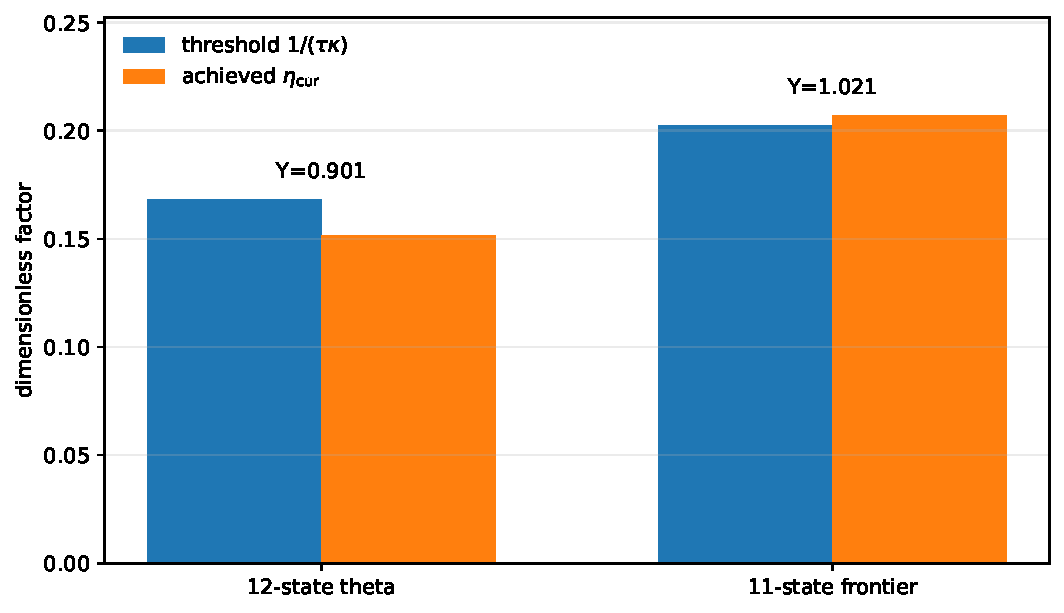
\includegraphics[width=0.82\linewidth]{figures/fig3_factor_threshold.pdf}
\caption{Current-weighted localization versus the violation threshold. A violation requires $\ecur<1/(\tau\kappa)$. The valid 11-state frontier misses the crossing by about $2.1\%$.}
\label{fig:factor-threshold}
\end{figure}

\section{Canonical 12-state theta counterexample}
The support graph is the theta graph between states 2 and 9 with paths
\begin{equation}
2-3-4-9,
\end{equation}
\begin{equation}
2-5-6-7-8-9,
\end{equation}
and
\begin{equation}
2-1-11-12-10-9.
\end{equation}
Thus $n=12$, the number of undirected edges is $m=13$, and the cycle rank is $m-n+1=2$. The exact positive integer rates are listed in Appendix~\ref{app:rates}.

\begin{figure}[t]
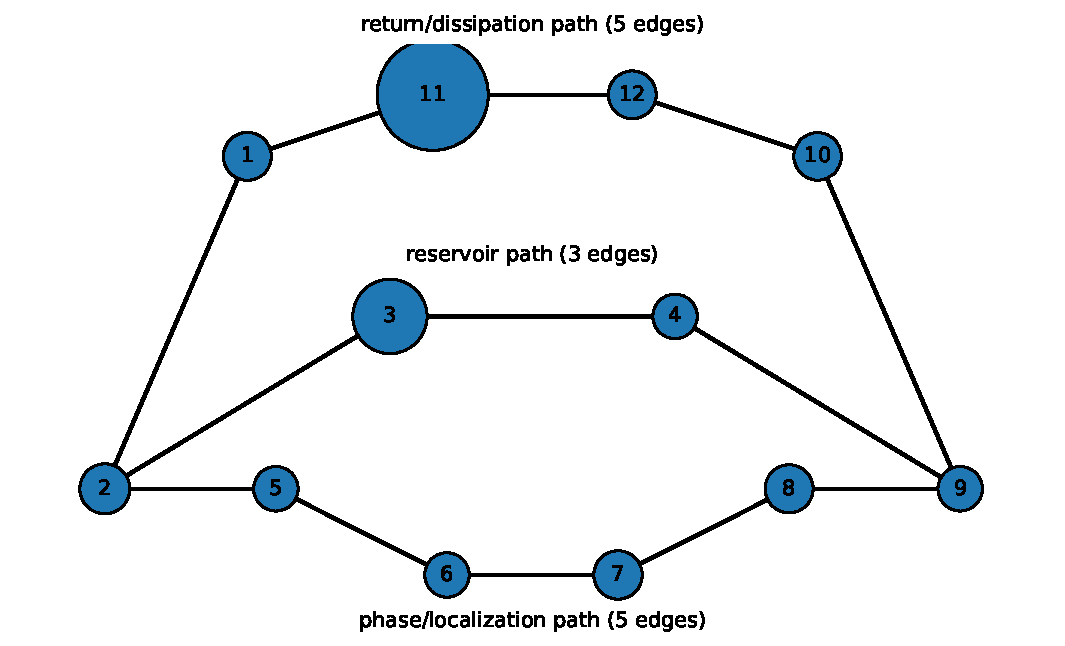
\includegraphics[width=0.8\linewidth]{figures/fig1_theta_topology.pdf}
\caption{Support of the exact 12-state counterexample. Node areas are scaled qualitatively by stationary mass. Branchwise diagnostics suggest a separation among stationary-mass storage, phase localization, and current return/dissipation; this assignment is interpretive rather than a necessary theorem.}
\label{fig:theta}
\end{figure}

\begin{theorem}[Certified theta counterexample]
The generator in Appendix~\ref{app:rates} is irreducible, has bidirectional support and exact rank 11, and has a unique spectral-leading nonzero conjugate pair. Certified intervals enclose
\begin{align}
\lambda_R&=5769.6623334454462165\ldots,\\
\lambda_I&=5818.6826824376867756\ldots,\\
\sigma&=5288.2047942788921693\ldots,
\end{align}
with
\begin{align}
\lambda_I-\lambda_R&>49.02034899224,\\
\glead&>41.72709294659,\\
Y&=0.90117537259574784327\ldots<1,\\
\Ncoh&=0.1605071592881499\ldots,\\
\Delta S&=5.710359625737439\ldots.
\end{align}
The ratio $\lambda_I/\lambda_R=1.008496224936437\ldots$ lies strictly but narrowly above the OBS visibility boundary. The backward-mode amplitude has a unique maximum at state 5, and Gu's factor is $\eta=0.0088589059175755\ldots$.
\end{theorem}

The coherence value is only $0.001352216196\ldots$ above the exact threshold $(2\pi)^{-1}$. The theorem therefore falsifies the conjecture in its stated unrestricted domain but does not establish failure for oscillators coherent over one or more full cycles. Because every listed rate is positive on the fixed support, the leading pair is simple, and the visibility, leadership, and violation inequalities have strict margins, continuity implies an open neighborhood of nearby generators with the same qualitative properties. The witness is thus not an isolated rational point, although no chemically calibrated realization is claimed.

The complete spectrum is isolated with Arb/Acb ball arithmetic. The nearest competing pair is
\begin{equation}
-5811.389426392041\ldots\pm i\,60.220759297817\ldots,
\end{equation}
which is almost real and only $41.727\ldots$ farther left than the target pair.

\begin{figure}[t]
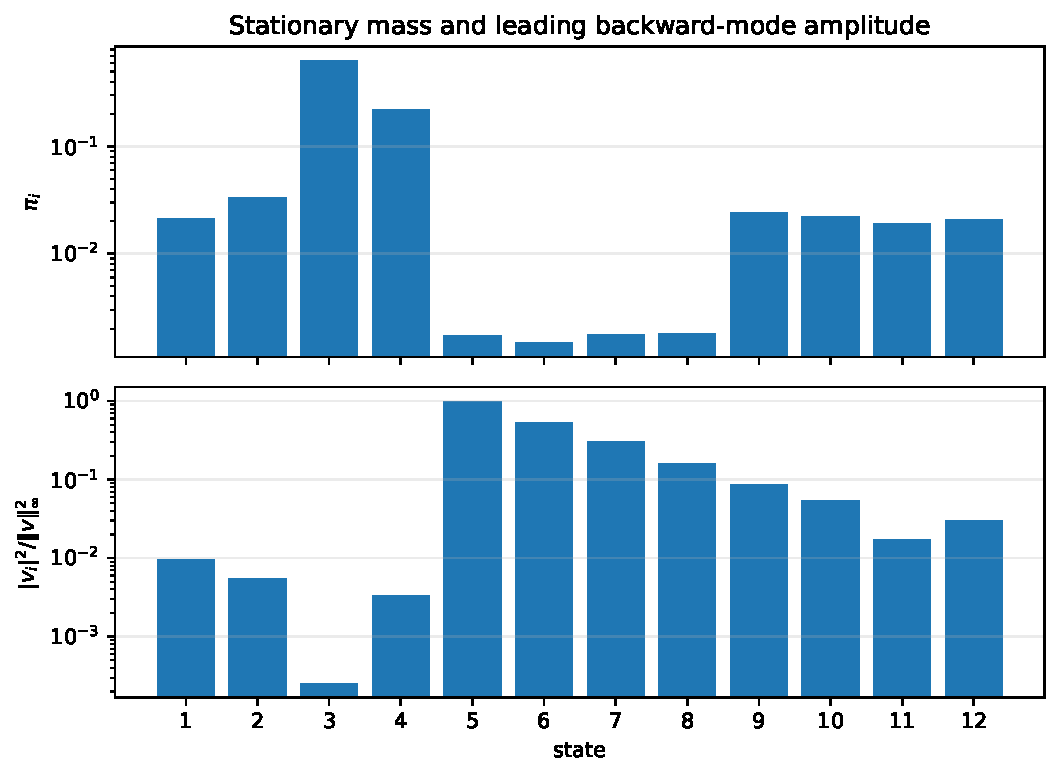
\includegraphics[width=0.85\linewidth]{figures/fig2_mass_mode_localization.pdf}
\caption{Stationary probability and normalized squared amplitude of the leading backward eigenmode. States 3 and 4 contain about $85.2\%$ of the stationary mass, while the mode peaks at state 5 in a low-mass sector.}
\label{fig:localization}
\end{figure}

\section{Witness diagnostics and branchwise division of labor}
The support makes the certified mechanism easier to diagnose. High-precision current and mode decomposition gives Table~\ref{tab:roles}. These percentages describe one exact witness and are not promoted as a necessary decomposition for all violations. The theorem-level mechanism is the current-weighted factorization and the matched-subdivision spectral intervention; the path-role language below is an explanatory diagnostic only.

\begin{table}[t]
\caption{Path roles in the 12-state theta witness. Fractions refer to internal stationary mass, target-mode norm, current--phase coupling $B$, and entropy production.}
\label{tab:roles}
\begin{ruledtabular}
\begin{tabular}{lrrrr}
path & mass & $\Nv$ & $B$ & entropy\\
\hline
$2-3-4-9$ & 0.852 & 0.100 & 0.085 & 0.171\\
$2-5-6-7-8-9$ & 0.0068 & 0.377 & 0.403 & 0.104\\
$2-1-11-12-10-9$ & 0.083 & 0.266 & 0.512 & 0.724\\
\end{tabular}
\end{ruledtabular}
\end{table}

The short path stores most of the stationary mass. The lower long path carries a large fraction of the rotating mode and useful phase coupling despite negligible mass. The upper long path carries most of the entropy production and more than half of $B$. For this witness, the network therefore exhibits a strong separation among stationary-mass storage, phase rotation, and thermodynamic return current. This branchwise pattern helps explain the small $\ecur$ factor, but the paper does not claim that the same assignment is necessary in every counterexample.

The 11-state search clarifies the remaining constraint. Some 11-state descendants already contain nonleading modes with $Y<1$, while the best valid 11-state system has $Y=1.021418567\ldots$ and an extremely small positive leading gap. The obstruction is therefore not the existence of a low-dissipation rotating mode; it is keeping that mode ahead of a localized relaxation competitor.

\section{Matched subdivision as a dynamic spectral spacer}
We now isolate the role of state 12. Contract the segment $11\leftrightarrows12\leftrightarrows10$ into a single bidirectional edge. The exact contracted rates are
\begin{equation}
k_{11,10}=\frac{765968}{15531},\qquad
k_{10,11}=\frac{201090092}{15531}.
\end{equation}
The contraction has 11 states, 12 edges, cycle rank two, and no additional chord. It is distinct from the separately reoptimized 11-state frontier discussed above.

For $s>0$, replace the contracted edge by the two-edge segment
\begin{align}
k_{11,12}&=977, & k_{12,11}&=\frac{14747}{15531}s,\\
k_{12,10}&=\frac{784}{15531}s, & k_{10,12}&=13636,
\end{align}
with all other rates fixed. The exact witness occurs at $s=15531$.

More generally, replacing an edge with rates $p,q$ by a state $x$ with
\begin{equation}
p_1=\frac p\alpha,\quad q_1=(1-\alpha)s,\quad
p_2=\alpha s,\quad q_2=\frac q{1-\alpha}
\end{equation}
produces the exact boundary-response identity
\begin{equation}
\boxed{A_{\rm sub}(z)-A_{\rm edge}(z)=\frac{z}{z+s}R_\alpha},
\qquad \mathrm{rank}(R_\alpha)=1.
\label{eq:spacer}
\end{equation}
The correction vanishes at $z=0$. The unnormalized stationary path current, total affinity, segment entropy production, and zero-frequency endpoint response are independent of $s$. The normalized stationary law changes only through the inserted state's exactly known mass:
\begin{equation}
\pi_i(s)=\frac{s\pi_i^{\rm con}}{s+C_0},\qquad
\pi_{12}(s)=\frac{C_0}{s+C_0}.
\end{equation}
Thus the intervention is statically matched but dynamically nontrivial.

\begin{theorem}[Certified causal window]
For every
\begin{equation}
15530\le s\le15532,
\end{equation}
the matched-subdivision generator is irreducible and has a unique spectral-leading visible conjugate pair continuously connected to the target branch of the exact contraction. Uniform exact/interval bounds give
\begin{align}
\lambda_I-\lambda_R&>47.020348992241,\\
\glead&>39.727092946595,\\
Y&<0.901947534017196<1.
\end{align}
At the contraction endpoint $s=\infty$, the same labeled target satisfies $Y<0.895963$ but
\begin{equation}
\lambda_I-\lambda_R<-265.268118377784,
\end{equation}
and
\begin{equation}
\glead<-590.961379909750.
\end{equation}
Moreover, the target remains invisible for every $s\ge158828$.
\end{theorem}

The proof is uniform, not a grid search. Eleven pairwise disjoint rational Rouch\'e disks each contain exactly one nonzero root throughout the closed valid interval, while the stationary root is controlled separately. A 17-link chain of overlapping exact parameter intervals in $t=1/s$ connects the contraction target to the finite-window target without relabeling roots by sorted eigenvalues. An independent exact rational similarity transformation with fixed disjoint Gershgorin disks certifies the wider interval $15528.9\le s\le15533.1$.

These intervals are conservative regions on which complete uniform proofs were carried out; they are not asserted to be the maximal valid window. The strict margins imply a local open neighborhood in the full positive-rate space around every certified point. High-precision continuation outside the proved bands is shown only as diagnostic evidence. Independently, the fixed-profile role-layer construction in Sec.~VIII produces certified violations for five distinct path lengths $L=5,\ldots,9$, providing a separate robustness check beyond the one-parameter inherited-edge slice.

\begin{figure}[t]
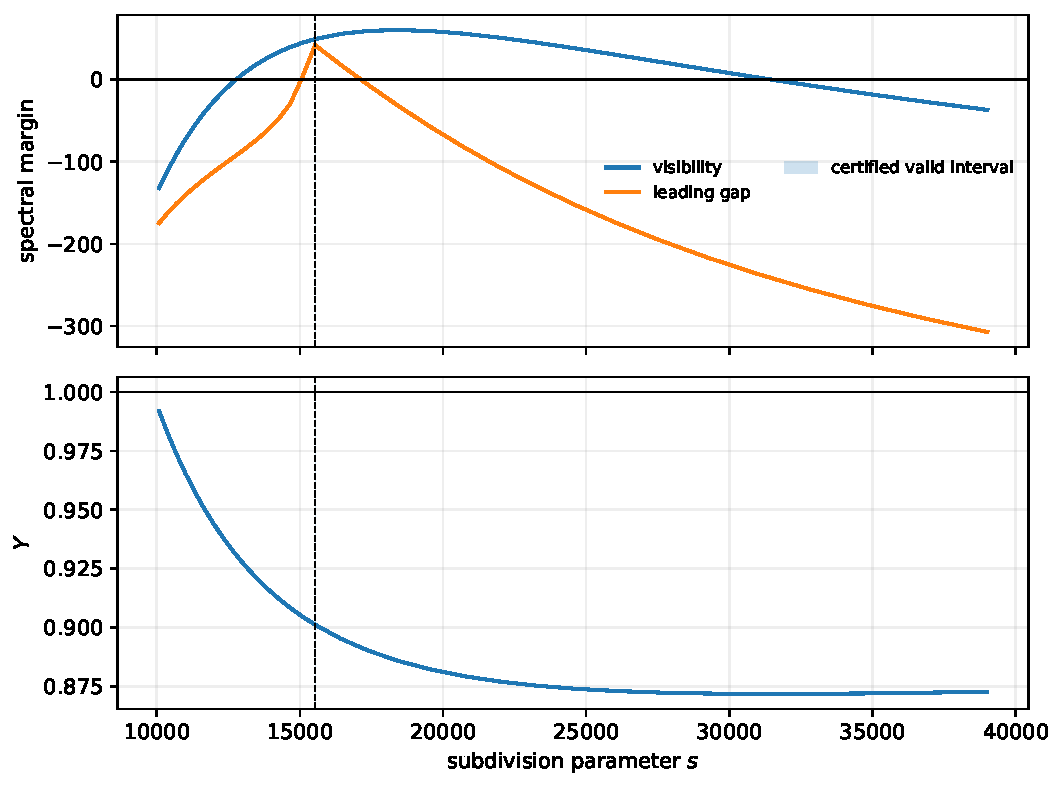
\includegraphics[width=0.86\linewidth]{figures/fig4_causal_window.pdf}
\caption{High-precision numerical continuation of visibility, global leading gap, and $Y$ along the matched-subdivision family. The narrow shaded band $15530\le s\le15532$ is the uniformly certified interval; the curves outside it are diagnostic numerical continuation. The dashed line is the integer witness $s=15531$.}
\label{fig:causal}
\end{figure}

The causal conclusion is precise. The 11-state contraction already contains the thermodynamically favorable rotating branch, but a slower relaxation mode dominates it. The inserted state supplies a rank-one frequency-dependent response that restores visibility and leadership without being needed to create $Y<1$. In this witness lineage, state 12 is a \emph{dynamic spectral spacer}.

\section{Global mode geometry and exceptional-point competitors}
For a general matched subdivision written with $\varepsilon=s^{-1}$, the reduced boundary matrix has the form
\begin{equation}
S(z,\varepsilon)=S_0(z)+\frac{\varepsilon z}{1+\varepsilon z}cd^{\mathsf T}.
\end{equation}
If $z_j(\varepsilon)$ is a simple root and $x_j,y_j$ are right and left boundary null vectors, differentiation gives
\begin{equation}
\frac{dz_j}{d\varepsilon}
=-\frac{\frac{z_j}{(1+\varepsilon z_j)^2}(y_j^{\mathsf T}c)(d^{\mathsf T}x_j)}
{y_j^{\mathsf T}\left[S_0'(z_j)+\frac{\varepsilon}{(1+\varepsilon z_j)^2}cd^{\mathsf T}\right]x_j}.
\label{eq:susceptibility}
\end{equation}
Equation~\eqref{eq:susceptibility} shows that the sign of relative target--competitor motion depends on global left/right mode couplings and Evans derivatives, not on the local path data alone.

\begin{proposition}[No local-invariants-only sign theorem]
There exist two exact irreducible three-state Markov contexts with identical matched edge rates, stationary distribution, edge current, traffic, affinity, inserted-mass law, and zero-frequency response, but with opposite signs of the real root motion under matched subdivision.
\end{proposition}
The explicit contexts and algebra are given in Appendix~\ref{app:local-obstruction}. This rules out an unconditional local form of the spectral-spacer theorem. Any generalization must retain global adjoint-mode or Evans-residue information.

The active competitor in the theta lineage is associated with the generic collision of two real relaxation roots. Near a real exceptional point $(z_*,\varepsilon_*)$ satisfying $E=E_z=0$ and $E_{zz}E_\varepsilon\ne0$, Weierstrass preparation gives the Puiseux law \cite{Kato1995}
\begin{equation}
z_\pm(\varepsilon)=z_*\pm
\sqrt{-2\frac{E_\varepsilon}{E_{zz}}(\varepsilon-\varepsilon_*)}
+O(\varepsilon-\varepsilon_*).
\end{equation}
The square-root sensitivity explains why a nearly real pair can abruptly overtake or release the rotating target. The certified causal interval itself does not cross an exceptional point; all roots remain isolated there.

\section{A fixed-profile robustness test: the role-layer family}
To test whether the phenomenon extends beyond a single inherited edge profile, we construct a constant-complexity $\Theta_{3,L,L}$ role-layer family. This section is a certified finite robustness study, not yet an open-box analytic-family theorem. The family uses 15 rational parameters independent of $L$: five mass roles, two independent path currents, and seven traffic roles, with one global rate-scale redundancy. No independently optimized rate array grows with path length.

At one fixed rational parameter profile, exact characteristic polynomials, rational Rouch\'e disks, and rigorous logarithm bounds classify lengths $L=3,\ldots,12$:
\begin{itemize}
\item $L=3,4$: the target is not visible;
\item $L=5,6,7,8,9$: certified OBS counterexamples;
\item $L=10,11,12$: visible and leading, but $Y>1$.
\end{itemize}
For $L=5$, the certified value is $Y<0.893201865220479$, with visibility $>59.21728$ and leading gap $>43.58682$. The result establishes a finite Goldilocks window in this explicit profile, but does not yet prove failure for every $L\ge10$ or provide an explicit positive-width rational box in all family parameters.

\begin{figure}[t]
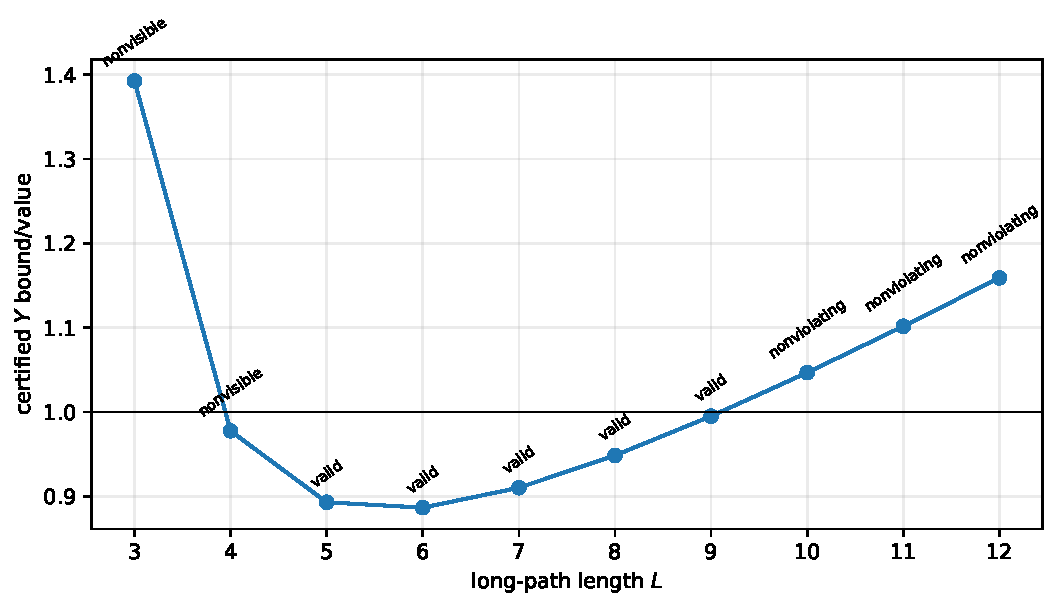
\includegraphics[width=0.84\linewidth]{figures/fig5_role_length_window.pdf}
\caption{Exact fixed-profile classification of the role-layer $\Theta_{3,L,L}$ family. Short paths fail visibility, intermediate paths violate, and the tested longer paths remain visible and leading but cross above $Y=1$.}
\label{fig:length}
\end{figure}

\section{Certification architecture}
The promoted claims are supported by deliberately different proof routes.
\begin{enumerate}
\item The theta witness checker constructs the generator over $\mathbb Q$, proves rank 11 and positivity of the stationary law, evaluates entropy with Arb, and isolates the full spectrum with Acb ball arithmetic \cite{Johansson2017}.
\item An independent audit reconstructs stationary weights by exact principal cofactors and isolates roots of the exact characteristic polynomial rather than reusing the matrix eigensolver.
\item A structural checker independently verifies the backward eigenvector, unique amplitude peak, currents, edgewise entropy, and the identities used in the factorization.
\item The causal-window proof uses uniform rational Rouch\'e disks over a parameter interval. The independent route uses an exact $\mathbb Q(i)$ similarity and fixed Gershgorin disks, without an eigensolver.
\item Hostile reconstruction checks generator orientation, entropy conventions, branch identity, complete root count, and the distinction between the exact 11-state contraction and the separately reoptimized 11-state frontier.
\item The symbolic paper core is formalized in Lean 4.29.0 against Mathlib. The machine-checked layer includes the current-weighted factorization, $\tau>1$, $\kappa>1$, $Y>\ecur\ge\eta$, the equality condition for $\ecur=\eta$, the matched-subdivision parameterization and response identity, and the exact local-sign obstruction. A clean pinned build completes 8,275 jobs with no warnings, errors, or proof-bypass declarations. The exact 12-state spectrum, Arb/Acb entropy bounds, Rouch\'e causal window, and role-layer length certificates remain external validated-computation claims rather than Lean claims.
\end{enumerate}
All exact inputs, checkers, Lean sources, build transcripts, theorem crosswalks, and SHA-256 manifests accompany the manuscript.

\section{Discussion}
The OBS conjecture fails because the leading eigenvalue and total entropy production do not determine how the oscillatory mode is distributed relative to the irreversible current network. The exact factorization
\begin{equation}
Y=\tau\kappa\ecur
\end{equation}
separates three questions: how efficiently current produces entropy, how efficiently mode variation produces directed phase rotation, and whether mode amplitude is concentrated on current-carrying edges. The theta witness violates because the last factor is small enough to overcome the first two penalties.

The causal family sharpens the theorem-level mechanism. The twelfth state is not needed to create a mode with $Y<1$; the contraction already has one. It changes the finite-frequency boundary response so that the same branch becomes visible and leading. Consequently, a state can be invisible to a matched zero-frequency reduction while remaining indispensable to oscillatory spectral ordering. This observation is relevant to model reduction beyond the OBS problem: preserving stationarity, local current, affinity, segment entropy, and DC endpoint response does not guarantee preservation of the dominant oscillatory mode.

\subsection{Proven mechanism and witness interpretation}
The rigorous mechanism consists of three parts: the current-weighted identity and inequalities, the exact rank-one dynamic response of matched insertion, and the uniformly certified branch rescue in the specified family. The additional assignment of the three theta paths to mass storage, phase localization, and thermodynamic return is a diagnostic summary of Table~II. It is useful for interpreting this generator, but it is not assumed by the proofs and is not claimed as a universal architecture.

\subsection{Scope and limitations}
The counterexample is a valid finite-state stochastic-thermodynamic process but is not calibrated to a named biochemical reaction network. Its coherence number, $\Ncoh=0.160507\ldots$, lies close to the exact OBS threshold and far below the regime of clocks that remain coherent for one or more full periods. Accordingly, the paper resolves the unrestricted universal conjecture, not the physically stronger high-coherence question.

We also do not claim 12-state minimality, exclude an 11-state counterexample, prove graph-unicyclic safety, or establish that cycle rank two is necessary. The matched-subdivision theorem is witness-specific; Proposition 1 shows why a universal sign rule based only on the listed local invariants cannot hold. The role-layer study certifies the finite range $L=3,\ldots,12$ at one fixed rational profile, but it neither supplies a positive-width box in all family parameters nor proves an all-$L$ tail theorem. These are independent continuation problems rather than premises of the present disproof.

\section{Conclusion}
We have given a sparse exact 12-state theta-graph counterexample to the unrestricted Oberreiter--Barato--Seifert dissipation--coherence conjecture and identified a certified mechanism for this witness lineage. Current-weighted localization supplies a sharper structural factor, while a dynamically matched inserted state rescues the favorable rotating branch from a competing relaxation mode. The result is mathematically robust in certified parameter intervals and is reproduced in a separate fixed-profile family, but it lies near the visibility threshold and is not presented as a model of a specific biochemical clock. The high-coherence regime, structural minimality, and broader global spectral-spacer conditions remain open.

\appendix
\section{Exact transition rates}\label{app:rates}
For every row below, the two entries are $(k_{ij},k_{ji})$. All omitted off-diagonal rates vanish.
\begin{center}
\begin{longtable}{c@{\qquad}r@{\,,\,}l}
\toprule
edge & \multicolumn{2}{c}{rates}\\
\midrule
$1-2$ & 15300 & 1109\\
$1-11$ & 926 & 15880\\
$2-3$ & 13202 & 293\\
$2-5$ & 760 & 50\\
$3-4$ & 1873 & 4248\\
$4-9$ & 1313 & 1107\\
$5-6$ & 15169 & 426\\
$6-7$ & 17527 & 131\\
$7-8$ & 14581 & 85\\
$8-9$ & 15784 & 120\\
$9-10$ & 12514 & 826\\
$10-12$ & 13636 & 784\\
$11-12$ & 977 & 14747\\
\bottomrule
\end{longtable}
\end{center}

\section{Exact local obstruction to a local spectral sign rule}\label{app:local-obstruction}
Take a three-state row generator with local rates $0\to1=2$ and $1\to0=1$, and context rates
\begin{equation}
0\to2=a,\quad2\to0=b,\quad1\to2=c,\quad2\to1=d.
\end{equation}
The two contexts
\begin{equation}
R:(a,b,c,d)=(1,2,2,1),\qquad
L:(a,b,c,d)=(2,3,2,1)
\end{equation}
have the same uniform stationary law and therefore the same local forward flow $2/3$, backward flow $1/3$, current $1/3$, traffic 1, affinity $\log2$, and matched inserted-state mass $2/s$. For subdivision fraction $\alpha=1/2$, the exact reduced Evans data are
\begin{center}
\begin{tabular}{ccl}
& $P(z)$ & $A(z)$\\
\hline
$R$ & $z(z^2+9z+21)$ & $3z^2+22z+42$\\
$L$ & $z(z+5)(z+6)$ & $3z^2+26z+60$.
\end{tabular}
\end{center}
At exact contraction, $z'(0)=-zA(z)/P'(z)$. Hence the upper complex root in context $R$ has $\mathrm{Re}\,z'(0)=5/2>0$, while the root $z=-5$ in context $L$ has $z'(0)=-5<0$. Identical local stationary invariants therefore permit opposite root motions.

\section{Data and code availability}
The complete reproducibility materials for this work are available in the public GitHub repository \url{https://github.com/shawnjason/OBS-Dissipation-Coherence-Counterexample}. Versioned releases of the repository are preserved through Zenodo and linked from the Zenodo record for this paper. The repository contains the exact 12-state witness data, corrected spectral analysis, causal-window certificates, Lean 4 formalization, successful clean-build audit, manuscript source, figures, reproduction instructions, environment records, and SHA-256 manifests.

The validated numerical certificates require Python and \texttt{python-flint}. The Lean project is pinned to Lean 4.29.0 and Mathlib revision \texttt{8a178386ffc0f5fef0b77738bb5449d50efeea95}. Its umbrella build includes \texttt{rowMarkov\_paperCore}, \texttt{rowMarkov\_etaCur\_eq\_eta\_iff}, the matched-subdivision modules, and the exact local-obstruction module. A fresh independent clean build completed successfully with 8,275 jobs, zero warnings or errors, and no proof bypasses. Lean verifies the general symbolic theorems but does not verify the witness-specific spectrum, logarithmic interval evaluation, or causal-window root isolation; those claims are supported by separate exact and validated computational certificates in the same repository.

\section{Use of artificial intelligence}
OpenAI GPT-5.6 Sol Ultra and GPT-5.6 Thinking were used for computational search, theorem discovery, code generation, adversarial audit, synthesis, and manuscript preparation. The human author selected and framed the scientific problem, directed the research program, reviewed the exact packages and audits, reran certificates, determined the scientific claims, and accepts responsibility for the manuscript. No AI system is listed as an author.


\begin{thebibliography}{10}
\bibitem{BaratoSeifert2017} A. C. Barato and U. Seifert, ``Coherence of biochemical oscillations is bounded by driving force and network topology,'' Phys. Rev. E \textbf{95}, 062409 (2017), \href{https://doi.org/10.1103/PhysRevE.95.062409}{doi:10.1103/PhysRevE.95.062409}.
\bibitem{OBS2022} L. Oberreiter, U. Seifert, and A. C. Barato, ``Universal minimal cost of coherent biochemical oscillations,'' Phys. Rev. E \textbf{106}, 014106 (2022), \href{https://doi.org/10.1103/PhysRevE.106.014106}{doi:10.1103/PhysRevE.106.014106}.
\bibitem{Gu2026} J. Gu, ``Dissipation-coherence tradeoff for stochastic oscillations,'' Phys. Rev. E \textbf{113}, 064130 (2026), \href{https://doi.org/10.1103/zxw1-zdb7}{doi:10.1103/zxw1-zdb7}.
\bibitem{Kolchinsky2026} A. Kolchinsky, ``Elementary derivation of the dissipation-coherence bound for stochastic oscillators,'' Phys. Rev. E, accepted 2 June 2026, \href{https://doi.org/10.1103/yj2t-frgz}{doi:10.1103/yj2t-frgz}.
\bibitem{XuEtAl2025} G.-H. Xu, A. Kolchinsky, J.-C. Delvenne, and S. Ito, ``Thermodynamic geometric constraint on the spectrum of Markov rate matrices,'' arXiv:2507.08938 (2025), \href{https://doi.org/10.48550/arXiv.2507.08938}{doi:10.48550/arXiv.2507.08938}.
\bibitem{KolchinskyOhgaIto2026} A. Kolchinsky, N. Ohga, and S. Ito, ``Cycle affinity and winding localize eigenvalues of Markov generators,'' arXiv:2605.15884 (2026), \href{https://doi.org/10.48550/arXiv.2605.15884}{doi:10.48550/arXiv.2605.15884}.
\bibitem{Schnakenberg1976} J. Schnakenberg, ``Network theory of microscopic and macroscopic behavior of master equation systems,'' Rev. Mod. Phys. \textbf{48}, 571--585 (1976), \href{https://doi.org/10.1103/RevModPhys.48.571}{doi:10.1103/RevModPhys.48.571}.
\bibitem{Seifert2012} U. Seifert, ``Stochastic thermodynamics, fluctuation theorems and molecular machines,'' Rep. Prog. Phys. \textbf{75}, 126001 (2012), \href{https://doi.org/10.1088/0034-4885/75/12/126001}{doi:10.1088/0034-4885/75/12/126001}.
\bibitem{Johansson2017} F. Johansson, ``Arb: Efficient arbitrary-precision midpoint-radius interval arithmetic,'' IEEE Trans. Comput. \textbf{66}, 1281--1292 (2017), \href{https://doi.org/10.1109/TC.2017.2690633}{doi:10.1109/TC.2017.2690633}.
\bibitem{Kato1995} T. Kato, \textit{Perturbation Theory for Linear Operators}, 2nd ed. (Springer, 1995), \href{https://doi.org/10.1007/978-3-642-66282-9}{doi:10.1007/978-3-642-66282-9}.
\bibitem{Lean4} L. de Moura and S. Ullrich, ``The Lean 4 theorem prover and programming language,'' in \textit{Automated Deduction---CADE 28}, Lecture Notes in Computer Science Vol. 12699 (Springer, 2021), pp. 625--635, \href{https://doi.org/10.1007/978-3-030-79876-5_37}{doi:10.1007/978-3-030-79876-5\_37}.
\bibitem{Mathlib} The mathlib Community, ``The Lean mathematical library,'' in \textit{Proceedings of the 9th ACM SIGPLAN International Conference on Certified Programs and Proofs} (ACM, 2020), pp. 367--381, \href{https://doi.org/10.1145/3372885.3373824}{doi:10.1145/3372885.3373824}.
\end{thebibliography}
\end{document}
